\section{Cryptographic Protocol}

\subsection{Classical Component: X25519 ECDH}
The X25519 algorithm is used as the standard key exchange algorithm~\cite{rfc7748}. The devices generate private and public keys for themselves, share the public key with the other side, and finally have the same shared secret on both ends. No secret information is ever transferred over the network.

\subsection{Post-Quantum Component: ML-KEM (Kyber-768)}
Additionally, there is Kyber, which is the quantum-resistant part of the construction~\cite{fips203}. This algorithm enables sending a secret from one device to another device with the help of the latter's public key. The secret is reconstructed locally, rather than being transmitted in its raw form. This adds an additional level of security to the application.

\subsection{Hybrid Key Derivation}
The app merges two shared secrets into a single session key using HKDF-SHA256~\cite{pqxdh}. The reasoning behind the approach is straightforward: if at least one protocol remains secure, the resulting key is also secure.

% \begin{verbatim}
% // Hybrid key setup
% ecdhSecret  = X25519(myPrivateKey, peerPublicKey)
% kyberSecret = Kyber.decapsulate(peerKyberCiphertext, myKyberSecret)
% sessionKey  = HKDF_SHA256(ecdhSecret || kyberSecret)
% \end{verbatim}

The algorithm above describes the key agreement algorithm used by the app. First, classical and post-quantum secret keys are mixed, and then merged into one session key.

It is an interesting compromise that the application prototype utilizes. Instead of trying to completely change all legacy protocols overnight, it uses two parallel approaches and thus gets to enjoy benefits of both classical and post-quantum cryptography at once.

\subsection{Symmetric Message Cipher: AES-256-GCM}
After the session key is established, the app protects the messages using AES-256-GCM~\cite{gcm}. This provides both confidentiality and integrity.

During each exchange of messages, the following occurs:
\begin{enumerate}
    \item Nonce is generated per message.
    \item Encryption and tagging.
    \item Transmission of the ciphertext and tag.
\end{enumerate}
Upon receiving the message, the other party reconstructs the message from its ciphertext, validates the tag, and decrypts the message. If validation fails, the message is simply ignored.

It is an important step since mere encryption is not enough for a chat app: besides encrypting messages, a chat must be able to detect any modifications of the message during the transmission process. Using GCM mode of AES allows us to get both encryption and message integrity.

\subsection{Atomic Role-Assignment Handshake}
To establish the first chat session, we need the devices to coordinate and pick their roles. We do this using Firestore transaction to ensure that no two devices will try to initiate a chat at the same time. The idea is illustrated in Fig.~\ref{fig:handshake}.
\begin{figure}[htbp]
\centering
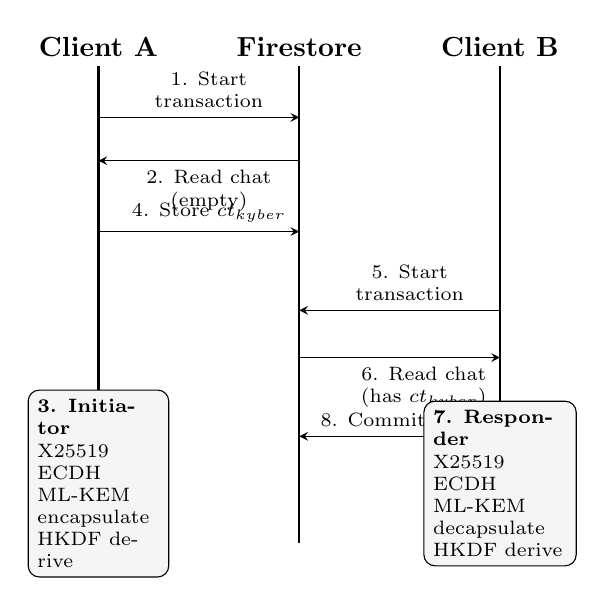
\begin{tikzpicture}[>=stealth, font=\scriptsize]
  \node[font=\bfseries] (A) at (0,0) {Client A};
  \node[font=\bfseries] (S) at (2.55,0) {Firestore};
  \node[font=\bfseries] (B) at (5.1,0) {Client B};

  \draw[thick] (A) -- (0,-6.3);
  \draw[thick] (S) -- (2.55,-6.3);
  \draw[thick] (B) -- (5.1,-6.3);

  \draw[->] (0,-0.9) -- node[above, pos=0.55, align=center] {1. Start\\transaction} (2.55,-0.9);
  \draw[->] (2.55,-1.45) -- node[below, pos=0.45, align=center] {2. Read chat\\(empty)} (0,-1.45);
  \draw[->] (0,-2.35) -- node[above, pos=0.55] {4. Store $ct_{kyber}$} (2.55,-2.35);

  \draw[->] (5.1,-3.35) -- node[above, pos=0.45, align=center] {5. Start\\transaction} (2.55,-3.35);
  \draw[->] (2.55,-3.95) -- node[below, pos=0.62, align=center] {6. Read chat\\(has $ct_{kyber}$)} (5.1,-3.95);
  \draw[->] (5.1,-4.95) -- node[above, pos=0.45] {8. Commit session} (2.55,-4.95);

  \node[draw, rounded corners, fill=gray!8, align=left, text width=1.55cm] at (0,-5.55) {
    \textbf{3. Initiator}\\
    X25519 ECDH\\
    ML-KEM encapsulate\\
    HKDF derive
  };
  \node[draw, rounded corners, fill=gray!8, align=left, text width=1.7cm] at (5.1,-5.55) {
    \textbf{7. Responder}\\
    X25519 ECDH\\
    ML-KEM decapsulate\\
    HKDF derive
  };
\end{tikzpicture}
\caption{Sequence diagram of the hybrid key exchange handshake mediated by a Firestore transaction.}
\label{fig:handshake}
\end{figure}
One device starts the exchange first, stores the Kyber output, and the other device reads it and finishes the exchange. Both devices then arrive at the same session key, which is reused for that chat.
